\documentclass[a4paper,11pt]{article}
\usepackage[francais]{babel}
%% Prévu pour compiler avec lualatex
% \usepackage[utf8]{inputenc}
\usepackage{fontspec}
%\usepackage{libertine}
% \usepackage[T1]{fontenc}
\usepackage{graphicx}
\usepackage{fancyhdr}
\usepackage[top=2.5cm, bottom=2.5cm, left=2cm, right=2cm]{geometry}
\usepackage{listings}
\usepackage[utf8]{luainputenc}
\usepackage[hidelinks]{hyperref}
\usepackage{caption}

\lfoot{\bsc{Enseirb-Matmeca}}
\rfoot{Informatique --- 3\ieme{} année}

\pagestyle{fancy}
\begin{document}

\begin{titlepage}
  \begin{center}

    \begin{center}
      
\includegraphics[width=4cm]{EM.jpg}
    \end{center}

    \vspace*{1cm}
        
    \rule{0.75\linewidth}{0.7mm}\\[0.4cm]
    {\Huge Rapport TP2 --- MPI\\[0.4cm]}
    \rule{0.75\linewidth}{0.7mm} \\[1.5cm]

    {\Large Bazire \bsc{Houssin}\\Sylvain \bsc{Vaglica}\\Stéphane \bsc{Castelli}\\[2cm]}
    {\Large Mardi 5 Novembre 2013}
  \end{center}
\end{titlepage}

\tableofcontents
\clearpage
\section{Introduction}

\section{Présentation de l'algorithme}


\section{Topologie, répartition des données et communications}
 
\section{Performances}

\begin{figure}[h!]
  \centering
  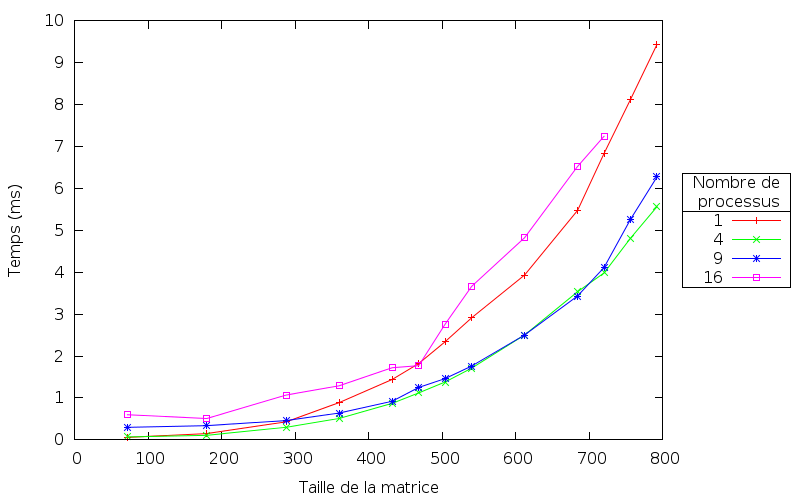
\includegraphics[width=\textwidth]{plot.png}
  \caption{Performance du programme}
  \label{perf}
\end{figure}


\section{Conclusion}


\end{document}
